\documentclass[10pt,a4paper]{article}
\usepackage[a4paper,margin=14mm,top=12mm,bottom=14mm]{geometry}
\usepackage{fontspec}
\setmainfont{Liberation Sans}
\usepackage{polyglossia}
\setdefaultlanguage{french}
\usepackage{amsmath}
\usepackage{xcolor}
\usepackage{graphicx}
\usepackage[most]{tcolorbox}
\usepackage{tabularx,booktabs,array,multirow}
\usepackage{enumitem}
\usepackage{fancyhdr}
\usepackage{lastpage}
\usepackage[hidelinks]{hyperref}
\definecolor{uimm}{HTML}{005677}
\definecolor{cyan}{HTML}{13A2DD}
\definecolor{fond}{HTML}{E6F2FA}
\definecolor{ok}{HTML}{2E7D32}
\definecolor{ko}{HTML}{B3261E}
\definecolor{violet}{HTML}{7B1FA2}
\setlength{\parindent}{0pt}
\setlength{\parskip}{3pt}
\setlist{nosep}
\setlist[itemize]{leftmargin=13pt,label=\textcolor{cyan}{\textbullet}}
\newcommand{\titre}[1]{\vspace{5pt}{\color{uimm}\large\bfseries #1}\par\vspace{-3pt}{\color{cyan}\rule{\linewidth}{1.2pt}}\par\vspace{0pt}}
\tcbset{boite/.style={colback=fond,colframe=uimm,boxrule=0.6pt,arc=2pt,left=6pt,right=6pt,top=4pt,bottom=4pt},
        defi/.style={colback=violet!6,colframe=violet,boxrule=0.8pt,arc=2pt,left=6pt,right=6pt,top=4pt,bottom=4pt,
                     title={\bfseries Défi},coltitle=white,colbacktitle=violet,fonttitle=\small}}
\newcommand{\bandeau}[3]{%
\begin{tcolorbox}[colback=uimm,colframe=uimm,arc=2pt,left=4pt,right=8pt,top=4pt,bottom=4pt]
\begin{minipage}[c]{18mm}\setlength{\fboxsep}{1.2pt}\fcolorbox{white}{white}{
\includegraphics[height=16.5mm]{logo_uimm.jpg}}\end{minipage}\hspace{4mm}%
\begin{minipage}[c]{\dimexpr\linewidth-22mm\relax}\color{white}
{\small #1}\\[1pt]{\LARGE\bfseries #2}\\[2pt]{\large #3}\hfill{\small CQPM Technicien qualité}
\end{minipage}
\end{tcolorbox}}
\newcommand{\reponse}[1][1]{\par\vspace{2pt}{\color{gray!60}\foreach \i in {1,...,#1}{\rule{\linewidth}{0.3pt}\par\vspace{9pt}}}}
\usepackage{pgffor}
\pagestyle{fancy}\fancyhf{}
\renewcommand{\headrulewidth}{0pt}
\newcommand{\pied}[1]{\fancyfoot[L]{\footnotesize\color{uimm}#1}\fancyfoot[R]{\footnotesize\color{uimm}Page \thepage{} sur \pageref{LastPage}}}

\usepackage{tikz}
\usepackage{longtable}
\renewcommand{\bandeau}[3]{%
\begin{tcolorbox}[colback=uimm,colframe=uimm,arc=2pt,left=4pt,right=8pt,top=4pt,bottom=4pt]
\begin{minipage}[c]{18mm}\setlength{\fboxsep}{1.2pt}\fcolorbox{white}{white}{
\includegraphics[height=16.5mm]{logo_uimm.jpg}}\end{minipage}\hspace{4mm}%
\begin{minipage}[c]{\dimexpr\linewidth-22mm\relax}\color{white}
{\small #1}\\[1pt]{\LARGE\bfseries #2}\\[2pt]{\large #3}
\end{minipage}
\end{tcolorbox}}
% en-tête d'une fiche : code, titre, question, bloc, durée, organisation, niveau
\newcommand{\entete}[7]{%
\begin{tcolorbox}[colback=uimm,colframe=uimm,arc=2pt,left=4pt,right=6pt,top=4pt,bottom=4pt]
\begin{minipage}[c]{18mm}\setlength{\fboxsep}{1.2pt}\fcolorbox{white}{white}{
\includegraphics[height=16.5mm]{logo_uimm.jpg}}\end{minipage}\hspace{3mm}%
\begin{minipage}[c]{\dimexpr\linewidth-58mm\relax}\color{white}\raggedright
{\small Base SPC · #4}\\[1pt]{\Large\bfseries #1 · #2}\\[2pt]{\itshape #3}
\end{minipage}\hfill
\begin{minipage}[c]{33mm}\color{white}\small\raggedleft
Durée : \textbf{#5}\\ \textbf{#6}\\ Niveau #7 sur 3
\end{minipage}
\end{tcolorbox}}
\newcommand{\tagE}{{\setlength{\fboxsep}{1.5pt}\colorbox{cyan}{\color{white}\scriptsize\bfseries Ellistat}}}
\newcommand{\tagW}{{\setlength{\fboxsep}{1.5pt}\colorbox{uimm}{\color{white}\scriptsize\bfseries Page web}}}
\tcbset{pred/.style={colback=orange!6,colframe=orange!80!black,boxrule=0.6pt,arc=2pt,left=6pt,right=6pt,top=3pt,bottom=1pt,
                    title={\bfseries Je prédis, avant de commencer},coltitle=white,colbacktitle=orange!80!black,fonttitle=\small},
        retenir/.style={colback=fond,colframe=uimm,boxrule=0.6pt,arc=2pt,left=6pt,right=6pt,top=3pt,bottom=3pt,
                    title={\bfseries À retenir},coltitle=white,colbacktitle=uimm,fonttitle=\small},
        plus/.style={colback=violet!6,colframe=violet,boxrule=0.6pt,arc=2pt,left=6pt,right=6pt,top=3pt,bottom=3pt,
                    title={\bfseries Pour aller plus loin},coltitle=white,colbacktitle=violet,fonttitle=\small},
        act/.style={colback=uimm!10,colframe=uimm,boxrule=0.5pt,arc=2pt,left=5pt,right=5pt,top=2pt,bottom=2pt,before skip=7pt,after skip=3pt},
        verif/.style={colback=orange!6,colframe=orange!80!black,boxrule=0.6pt,arc=2pt,left=6pt,right=6pt,top=3pt,bottom=3pt,
                    title={\bfseries À vérifier sur poste avant la première séance},coltitle=white,colbacktitle=orange!80!black,fonttitle=\small}}
\newcommand{\fichier}[1]{\texttt{\small #1}}
\newcommand{\menu}[1]{\textsf{\textbf{#1}}}
\newcommand{\champ}[1]{\rule{#1}{0.3pt}}

\usepackage{amssymb}
\newcommand{\cb}{$\square$\,}
\newcommand{\etape}[2]{\par\vspace{9pt}{\setlength{\fboxsep}{3pt}\colorbox{uimm}{\color{white}\bfseries\large\ #1\ }}\hspace{4pt}{\color{uimm}\large\bfseries #2}\par\vspace{2pt}}
\newcommand{\motnouveau}[1]{\begin{tcolorbox}[colback=violet!6,colframe=violet,boxrule=0.6pt,arc=2pt,left=6pt,right=6pt,top=3pt,bottom=3pt,title={\bfseries Mot nouveau},coltitle=white,colbacktitle=violet,fonttitle=\small]#1\end{tcolorbox}}
\newcommand{\chiffre}[1]{\begin{tcolorbox}[colback=orange!8,colframe=orange!80!black,boxrule=1pt,arc=3pt,left=8pt,right=8pt,top=5pt,bottom=5pt]#1\end{tcolorbox}}

\usepackage{colortbl}
\pied{Bachelor Maintenance · TP 2 · La carte u des pannes · Guide formateur et corrigé}
\newcommand{\src}[1]{{\footnotesize\color{uimm}\textit{Source : #1}}}
\begin{document}
\thispagestyle{fancy}
\entete{TP 2}{Guide formateur et corrigé}{La carte u des pannes : exposition, dérive, règle d'alerte}{Cartes aux attributs · Fiabilité}{2 h 30}{7 Bachelor, binômes}{3}

\begin{tcolorbox}[boite]
\textbf{Pièces du dossier remis aux stagiaires.} \textbf{Pièce 1} : fiche stagiaire (4 pages, dont la fiche de collecte p. 4). \textbf{Pièce 2} : \fichier{Pannes\_cellule\_C2\_simule.xlsx} (78 semaines). \textbf{Pièce 3} : \fichier{Pannes\_parc\_presses\_simule.xlsx} (52 semaines). Chaque réponse du corrigé cite sa pièce et sa page.\par
\textbf{Objectifs.} (1) Compter des pannes en tenant compte de l'exposition. (2) Lire une carte u en phase I puis en surveillance. (3) Écrire un MTBF avec son intervalle de confiance. (4) Reconnaître la surdispersion et savoir pourquoi on regarde la carte U Laney. (5) Produire une règle d'alerte et une note de décision.\par
\textbf{Prérequis.} Stage fiabilité (MTBF, Weibull, courroies $\beta = 5{,}52$), stage SPC (cartes de mesures, notion de phase I). Les cartes aux attributs sont nouvelles pour le groupe.
\end{tcolorbox}

\begin{tcolorbox}[verif]
Les valeurs de ce guide sont recalculées par script (Python, séries simulées, graine fixée). Elles ne sont \textbf{pas} relevées sur l'écran d'Ellistat. À contrôler sur un poste avant la séance : (a) les limites de la carte u pour $h = 80$ h et $h = 120$ h correspondent à 0,1034 et 0,0914 ; (b) la carte c, tracée avec la valeur 1 dans « Taille de lot (si fixe) » (piège relevé dans le guide de la base : champ vide, 25 points seulement), affiche 78 points, $\bar c = 3{,}346$, limite 8,83, et signale les semaines 15, 60, 63, 67, 72 ; (c) la carte u signale 63, 67, 72, 78 ; (d) la carte U Laney sur la pièce 3 ne signale aucune semaine ; (e) Ellistat applique aussi des règles supplémentaires (même côté 9 points, tendance 7 points, 2 points sur 3 près des limites, alternance 15 points : voir le guide de la base) qui marquent des points en rouge pâle. Mon calcul approché sur la pièce 2 : rien en phase I ; en surveillance, 9 points du même côté de la moyenne à la semaine 78 (série 70 à 78) et « 2 points sur 3 au-delà de 2 écarts types » aux semaines 62, 63, 64, 72, 73, 77, 78. La définition exacte d'Ellistat n'est pas confirmée : la lecture à l'écran fait foi. Ces règles peuvent faire apparaître une alerte dès la semaine 62, soit un point plus tôt que la limite à 3 écarts types ;
(g) la semaine 37 de la pièce 3 est sous la limite basse de très peu (0,0148 contre 0,0151) : Ellistat peut l'afficher ou non ; (f) libellé exact de la fonction du khi-deux dans votre version du tableur. Si un écart apparaît, l'écran fait foi et ce guide est à corriger.
\end{tcolorbox}

\titre{Hypothèses des données simulées}
Série 1 (cellule C2, pièce 2) : taux de pannes de référence $\lambda_0 = 0{,}040$ par heure de marche (MTBF théorique 25 h, valeur du plan). Heures hebdomadaires : 40, 56, 80 ou 120 h. À partir de la \textbf{semaine 60}, le taux double (changement non annoncé aux stagiaires). Pannes tirées par une loi de Poisson d'espérance $\lambda \times h$. Série 2 (parc de 6 presses, pièce 3) : 52 semaines de 360 à 540 h, taux hebdomadaire variable d'une semaine à l'autre (coefficient de variation 30 \%), donc volontairement surdispersée. Les graines (37 et 5) ont été choisies pour que les cas pédagogiques apparaissent ; c'est un choix assumé, il faut le dire aux stagiaires en fin de séance (« la série est un exemple construit, pas un échantillon tiré au hasard »).

\titre{Déroulé (2 h 30)}
\begin{tabularx}{\linewidth}{|>{\raggedright\arraybackslash}p{27mm}|>{\centering\arraybackslash}p{14mm}|X|}
\hline
\rowcolor{fond}\textbf{Étape} & \textbf{Durée} & \textbf{Consigne formateur}\\\hline
Situation, prédiction & 10 min & Laisser répondre à la prédiction par écrit avant toute discussion. Ne pas corriger.\\\hline
Étapes 1 et 2 & 20 min & $\bar u$ à la main. Passer chez chaque binôme : \og pannes par heure\fg{} et \og pannes pour 100 h\fg{} ne sont pas la même unité.\\\hline
Étape 3, carte c & 15 min & Ellistat. Faire noter la semaine 15 sans commenter.\\\hline
Étape 4, carte u & 20 min & Comparer avec le calcul manuel. Faire expliquer la ligne brisée.\\\hline
Étape 5, MTBF et intervalle & 20 min & Le khi-deux est un outil, pas un cours : donner la formule, faire calculer.\\\hline
Étape 6, parc et U Laney & 25 min & Deux cartes, deux conclusions. Laisser le désaccord s'installer avant de l'expliquer.\\\hline
Étape 7, règle d'alerte & 15 min & Seuils en nombre de pannes, puis plan de réaction (qui, quand, quoi).\\\hline
Étape 8, note de décision & 20 min & Une page, rédigée individuellement. Ramasser.\\\hline
Débriefing & 5 min & Dévoiler la semaine 60 et la construction des séries.\\\hline
\end{tabularx}

\titre{Corrigé}
\begin{enumerate}[label=\textcolor{cyan}{\textbf{Q\arabic*.}},leftmargin=22pt,itemsep=5pt]
\item \textbf{Prédiction et Q1.} Semaine 15 : $u = 10/120 = 0{,}0833$ panne par heure. Semaine 78 : $u = 8/56 = 0{,}1429$. La semaine 78 est la plus préoccupante : son taux est 1,7 fois celui de la semaine 15 et dépasse sa limite (0,1162). La semaine 15 reste sous sa limite (0,0914). La plupart des stagiaires répondront « semaine 15, 10 pannes » : c'est le but de la prédiction. \src{Pièce 1, p. 1 (prédiction) et p. 2 (Q1) ; pièce 2, lignes 16 et 79.}
\item \textbf{Q2.} Phase I : $N = 174$ pannes, $T = 4\,576$ h, $\bar u = 0{,}03802$ panne/h, soit $3{,}80$ pannes pour 100 h, MTBF $= 1/\bar u = 26{,}3$ h. \src{Pièce 1, p. 2 (Q2) et p. 1 (étape 2) ; pièce 2, semaines 1 à 52.}
\item \textbf{Q3.} $h = 80$ h : $0{,}03802 + 3\sqrt{0{,}03802/80} = 0{,}1034$, soit 8,27 pannes. $h = 120$ h : $0{,}0914$, soit 10,97 pannes. Pour $h = 56$ h : $0{,}1162$ (6,5 pannes) ; pour $h = 40$ h : $0{,}1305$ (5,2 pannes). La limite inférieure est négative, donc ramenée à 0. \src{Pièce 1, p. 2 (Q3) et p. 1 (étape 2).}
\item \textbf{Q4, carte c.} Limite supérieure $= 3{,}346 + 3\sqrt{3{,}346} = 8{,}83$ pannes. Semaines hors limite : 15, 60, 63, 67, 72. La semaine 15 est en phase I : alarme sur un fonctionnement normal (10 pannes sur 120 h, $u = 0{,}0833$ sous sa limite). Ce n'est pas une panne anormale, c'est une semaine longue : 16 des 52 semaines de la phase I ont 120 h. \src{Pièce 1, p. 2 (Q4) ; pièce 2 ; figure 2 ci-dessous.}
\item \textbf{Q5, carte u.} Semaines hors limite : 63, 67, 72, 78 ; aucune en phase I. La limite $\bar u + 3\sqrt{\bar u/h}$ dépend de l'exposition $h$ de la semaine : plus la semaine est courte, plus un taux élevé est plausible par hasard, donc plus la limite est haute. \src{Pièce 1, p. 2 (Q5) ; figure 1 ci-dessous.}
\item \textbf{Q6, comparaison.} La carte c signale à tort la semaine 15 (fausse alarme), signale la semaine 60 (9 pannes sur 120 h, $u = 0{,}075$, sous la limite de la carte u) et ne signale pas la semaine 78 (8 pannes, sous 8,83 alors que 56 h de marche rendent ce taux anormal). Elle se trompe dans les deux sens, selon la longueur de la semaine. Pour un responsable maintenance, le signal manqué est plus grave que la fausse alarme : il retarde la réaction ; la fausse alarme coûte une analyse. Accepter les deux réponses argumentées. \src{Pièce 1, p. 2 (Q6) ; figures 1 et 2.}
\item \textbf{Q7, MTBF et intervalles à 95 \%.} Phase I : $\lambda = 0{,}03802$, intervalle $[0{,}0326 ; 0{,}0441]$, MTBF $26{,}3$ h, intervalle $[22{,}7 ; 30{,}7]$ h. Surveillance (semaines 53 à 78) : $N = 163$, $T = 2\,208$ h, $\lambda = 0{,}0738$, intervalle $[0{,}0629 ; 0{,}0861]$, MTBF $13{,}5$ h, intervalle $[11{,}6 ; 15{,}9]$ h. \src{Pièce 1, p. 2 (Q7) et p. 2 (étape 5) ; pièce 2.}
\item \textbf{Q8.} Phase I : 25 h appartient à $[22{,}7 ; 30{,}7]$, le plan est compatible. Surveillance : 25 h est au-dessus de la borne haute 15,9 h, le plan n'est plus valable. Les deux intervalles ne se recouvrent pas. Un test exact de comparaison de deux taux de Poisson, semaines 60 à 78 contre semaines 1 à 52, donne $p \approx 10^{-11}$ (rapport des taux 2,2). Pour le débriefing : le doublement date de la semaine 60 ; sur les semaines 60 à 78 seules, $\lambda = 0{,}0842$, MTBF $11{,}9$ h, intervalle $[10{,}0 ; 14{,}2]$ h. Les semaines 53 à 59 (29 pannes en 616 h) sont encore compatibles avec la référence : estimer sur 53 à 78 mélange deux régimes et sous-estime l'aggravation. \src{Pièce 1, p. 2 (Q8) ; pièce 2.}
\item \textbf{Q9, parc de presses.} Carte u : 4 semaines hors limite (4, 35 et 48 au-dessus, 37 au-dessous de justesse). Carte U Laney : aucune. Le test d'homogénéité donne $\chi^2 = 138{,}0$ pour 51 degrés de liberté ($p \approx 6 \times 10^{-10}$), soit un rapport de $2{,}71$ ; l'écart type corrigé de Laney est $\sigma_z = 1{,}68$ au lieu de 1. Le taux de pannes varie d'une semaine à l'autre bien plus que le hasard de Poisson ne l'explique (presses différentes, régimes différents), sans qu'une cause spéciale unique l'explique. Conclusion : ne pas chasser les 4 semaines une par une ; stratifier par presse avant de tirer une conclusion sur le parc. La carte U Laney ne dit pas « tout va bien » : elle dit que le bruit est structurel. \src{Pièce 1, p. 3 (Q9) ; pièce 3 ; figure 3.}
\item \textbf{Q10, carte stable et $\beta$.} Non. Une carte sans alarme est compatible avec un taux constant, elle ne le démontre pas : la puissance est faible. Avec la carte de la série 1 à 80 h par semaine, la probabilité d'alarme dans une semaine vaut 0,4 \% si le taux est inchangé, 4,3 \% s'il augmente de 50 \%, 16,2 \% s'il double (délai moyen de détection $\approx 6$ semaines), 56 \% s'il triple. Il manque aussi un examen des temps entre pannes (Weibull sur les intervalles par poste) : un parc dont les machines sont d'âges décalés peut avoir un taux global constant avec des machines qui s'usent. \src{Pièce 1, p. 3 (Q10 et « Pour aller plus loin ») ; tableau ci-dessous.}
\end{enumerate}

\begin{center}
\begin{tabularx}{0.95\linewidth}{|>{\centering\arraybackslash}X|>{\centering\arraybackslash}X|>{\centering\arraybackslash}X|>{\centering\arraybackslash}X|>{\centering\arraybackslash}X|}
\hline
\rowcolor{fond}\textbf{Taux réel / $\bar u$} & \textbf{1} & \textbf{1,5} & \textbf{2} & \textbf{3}\\\hline
$h = 80$ h : alarme par semaine & 0,4 \% & 4,3 \% & 16,2 \% & 56,1 \%\\\hline
$h = 80$ h : délai moyen (semaines) & 241 & 23,1 & 6,2 & 1,8\\\hline
$h = 120$ h : alarme par semaine & 0,7 \% & 8,8 \% & 30,9 \% & 80,3 \%\\\hline
$h = 120$ h : délai moyen (semaines) & 136 & 11,4 & 3,2 & 1,2\\\hline
\end{tabularx}\\[2pt]
{\footnotesize Règle unique : un point au-dessus de la limite (alarme si le nombre de pannes dépasse 8 pour 80 h, 10 pour 120 h). Calcul : loi de Poisson exacte. Les règles supplémentaires raccourcissent le délai.}
\end{center}

\titre{Étape 7 : règle d'alerte (réponse attendue)}
Alarme dès que le nombre de pannes de la semaine dépasse : 5 pour 40 h, 6 pour 56 h, 8 pour 80 h, 10 pour 120 h (c'est-à-dire à partir de 6, 7, 9 et 11). Plan de réaction attendu : alarme saisie par le responsable maintenance le lundi, liste des pannes de la semaine par poste et par cause sous 48 h, décision (analyse approfondie, stratification, intervention) et nouvelle estimation du taux après 4 semaines. La précision du calendrier est celle du stagiaire, pas du formateur ; ce qui compte est la présence d'un déclencheur chiffré, d'un responsable et d'un délai.

\begin{figure}[h]\centering
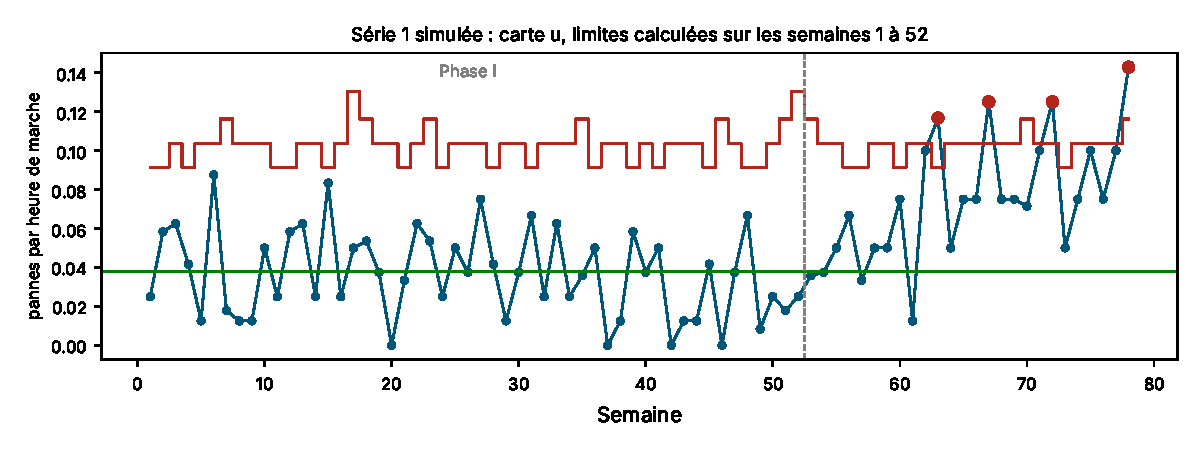
\includegraphics[width=0.92\linewidth]{u_s1.pdf}\\[-2pt]
{\footnotesize Figure 1 : carte u de la pièce 2 (limites calculées sur la phase I).}
\end{figure}
\begin{figure}[h]\centering
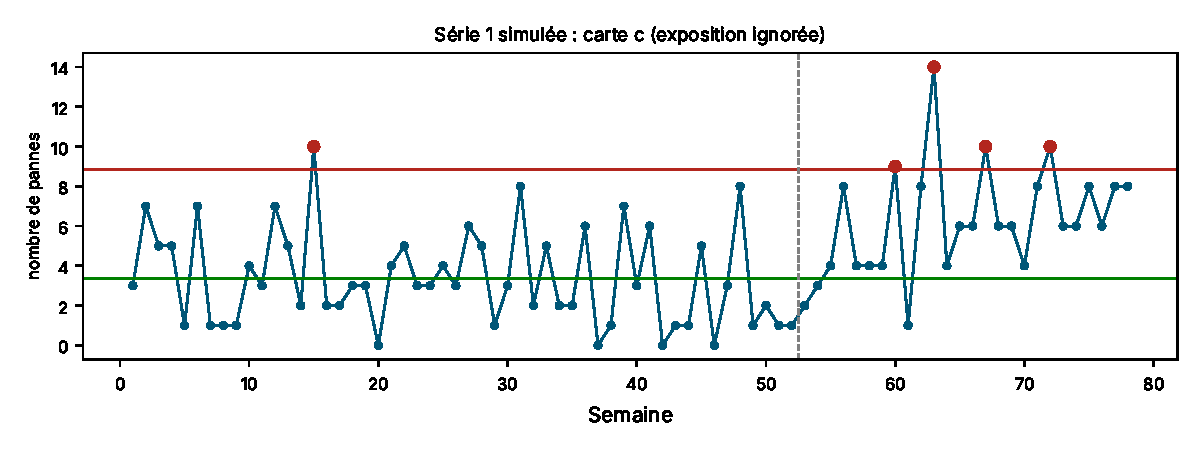
\includegraphics[width=0.92\linewidth]{c_s1.pdf}\\[-2pt]
{\footnotesize Figure 2 : carte c de la pièce 2 (exposition ignorée).}
\end{figure}
\begin{figure}[h]\centering
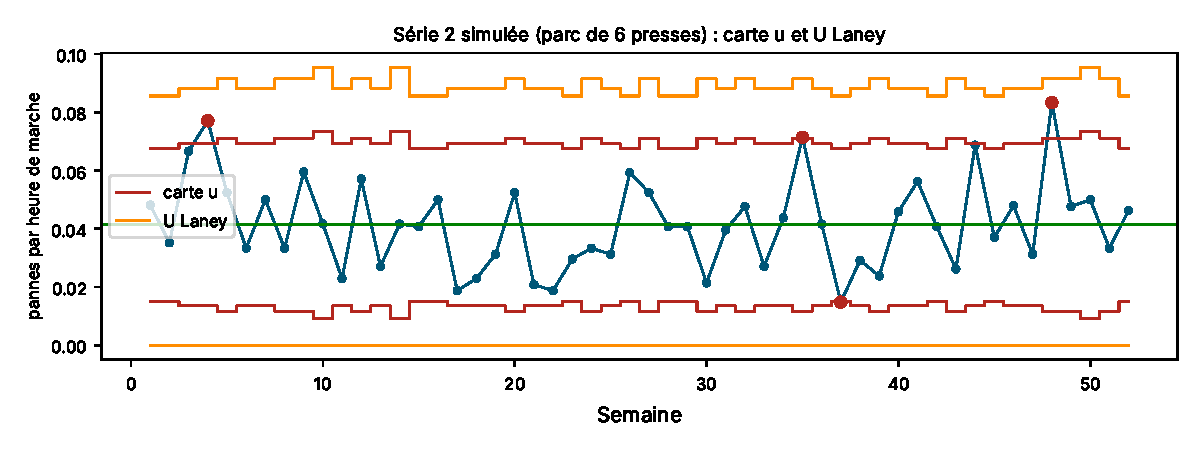
\includegraphics[width=0.92\linewidth]{u_s2.pdf}\\[-2pt]
{\footnotesize Figure 3 : cartes u et U Laney de la pièce 3. Ces figures sont tracées par script, l'affichage d'Ellistat peut différer.}
\end{figure}

\titre{Barème de la note de décision (sur 10)}
\begin{tabularx}{\linewidth}{|X|>{\centering\arraybackslash}p{14mm}|}
\hline
\rowcolor{fond}\textbf{Critère} & \textbf{Points}\\\hline
Réponse claire aux trois questions du directeur (réelle ou non, MTBF du plan, règle d'alerte) & 3\\\hline
Chiffres cités et corrects : $\bar u$, MTBF avec intervalle, semaines en alarme & 3\\\hline
Décision proposée justifiée (plan de maintenance, analyse des causes, stratification) & 2\\\hline
Limites de l'analyse énoncées (données simulées ou GMAO, définition de la panne, nombre de pannes, hypothèse de taux constant) & 2\\\hline
\end{tabularx}

\titre{Erreurs fréquentes}
\begin{itemize}
\item Oublier de vérifier la valeur de Fin en phase I : les limites sont alors calculées sur 78 semaines, avec la dérive incluse. Les alarmes changent.
\item Carte c : laisser « Taille de lot (si fixe) » vide : seuls 25 points sont tracés (saisir 1). Carte u : laisser ce champ vide, la limite forme une ligne brisée (comportement vérifié sur les 25 rouleaux de la fiche A7).
\item Donner un MTBF sans intervalle. Exiger la phrase : « entre \dots{} et \dots{} h à 95 \% ».
\item Écrire que la carte U Laney « supprime les fausses alarmes ». Elle corrige les limites quand le taux varie plus que le hasard, elle n'efface pas la cause de cette variation.
\item Lecture de $\bar u$ : pannes par heure ou pour 100 h ; ne pas additionner des moyennes de $u$ (moyenne des $u$ $\neq$ total des pannes sur total des heures).
\end{itemize}

\titre{Suite proposée}
TP 1 (carte XmR d'un indicateur vibratoire du banc BV12) : l'indicateur d'état détecte la dérive avant la panne, ce que le comptage des pannes ne peut pas faire ; on y reprend la notion de phase I et d'état de référence. TP 3 : capabilité du moyen de mesure (Cg, Cgk) sur pied à coulisse et micromètre. Les cartes aux attributs p et np (non-conformités en réception) viendront ensuite.

\titre{Vérification des chiffres}
Chaque nombre de ce guide a été recalculé en Python (numpy, scipy) à partir des fichiers de la pièce 2 et de la pièce 3. Les intervalles de Poisson ont été contrôlés indépendamment : pour chaque borne, la probabilité de queue de la loi de Poisson vaut bien 0,025. Le script est fourni avec les données (\fichier{gen\_series.py}).
\end{document}
